%%% První kapitola

\chapter{Definice a vlastnosti Jonesova polynomu}

Vhodné věci kurzívou, Zmínit původní definici?, Nekonzistentní používání V(t), V? Dvojtečky po platí

Původní definice Jonesova polynomu vycházela z operátorových algeber. A že tady to je na lincích.

Zapracovat, že je to z těch dvou knih a článku. Zmínit původní paper?
\section{Základní pojmy}
Jonesův polynom je invariant nejen uzlů, ale také linků, tedy více propletených uzlů. Pokud není řečeno jinak, pracujeme v textu s linky. 
Při definování Jonesova polynomu je důležité rozlišovat mezi linkem a jeho diagramem. Diagram je vhodné rovinné nakreslení nějaké linkové projekce, v němž je rozlišeno, jestli křížení vedou zvrchu nebo zespodu. Každý link má nekonečně mnoho diagramů.

V diagramu orientovaného linku rozlišujeme křížení s kladnou a zápornou orientací.

\begin{figure}[h]  
\centering 
\begin{subfigure}[t]{0.4\linewidth}\centering
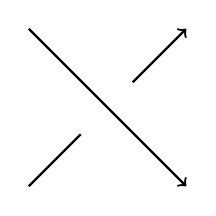
\begin{tikzpicture}[scale=2] 
\draw [thick] (0,0) -- (0.33,0.33);
\draw [thick,->] (0.66,0.66)-- (1,1);
\draw [thick,->] (0,1)  -- (1,0);
\end{tikzpicture} 
\caption{Kladná orientace} 
\end{subfigure}
\begin{subfigure}[t]{0.4\linewidth}\centering
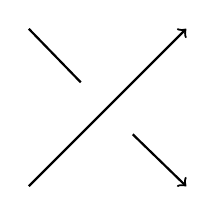
\begin{tikzpicture}[scale=2]
\draw [thick,->] (0,0) -- (1,1);
\draw [thick] (0,1) -- (0.33, 0.66);
\draw [thick,->] (0.66, 0.33) -- (1,0);
\end{tikzpicture}  
\caption{Záporná orientace}
\end{subfigure}
\caption{Orientace křížení}
\end{figure}  


Pro popis polynomů na uzlech a lincích se často používají \emph{skein vztahy} \footnote{česky přadenové vztahy}.
Skein vztahy určují, jaká je spojitost mezi polynomy tří linků $L_+$, $ L_-$ a $L_0$, jejichž diagramy jsou identické až na oblast jednoho křížení. V linku $L_+$ má toto křížení kladnou orientaci, v $L_-$ zápornou a v $L_0$ je křížení rozpojené.

\begin{figure}[h]  
\centering 
\begin{subfigure}[t]{0.4\linewidth}\centering
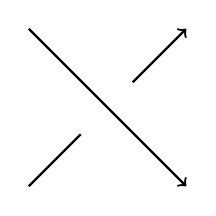
\begin{tikzpicture}[scale=2] 
\draw [thick] (0,0) -- (0.33,0.33);
\draw [thick,->] (0.66,0.66)-- (1,1);
\draw [thick,->] (0,1)  -- (1,0);
\end{tikzpicture} 
\caption{$L_+$} 
\end{subfigure}
\begin{subfigure}[t]{0.4\linewidth}\centering
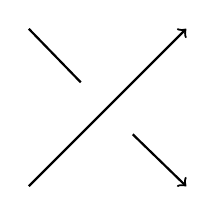
\begin{tikzpicture}[scale=2]
\draw [thick,->] (0,0) -- (1,1);
\draw [thick] (0,1) -- (0.33, 0.66);
\draw [thick,->] (0.66, 0.33) -- (1,0);
\end{tikzpicture}  
\caption{$L_-$}
\end{subfigure}
\begin{subfigure}[t]{0.4\linewidth}\centering
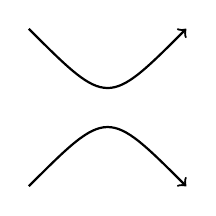
\begin{tikzpicture} [scale=2]
\draw  [thick,->](0,0) .. controls (1/2,1/2)  .. (1,0);
\draw  [thick,->](0,1) .. controls (1/2,1/2)  .. (1,1);
\end{tikzpicture}
\caption{$L_0$}
\end{subfigure}
\caption{Diagramy skein vztahu}
\end{figure}

\section{Definice}

\begin{definice}\label{def01:1}
\emph{Jonesův polynom} orientovaného linku $L$ je Laurentův polynom v proměnné $\sqrt t$ (tj. polynom v $\Z[t^{1/2}, t^{-1/2}]$), značený $V_L(t)$ , který:
\begin{enumerate}
\item
je linkový invariant,
\item 
  je normalizovaný, tedy polynom  $V_\circlearrowleft$, kde $\circlearrowleft$ je orientovaný triviální uzel, má hodnotu $1,$
\item  
splňuje skein vztah 
$$ \frac{1}{t} V_{L_+} - t V_{L_-} = (\sqrt{t}  - \frac{1}{\sqrt{t}}) V_{L_0}.$$
\end{enumerate}
\end{definice}

\begin{lemma}\label{l01:1}
Buď $L$ link, který se skládá z $k$ neprotínajících se orientovaných triviálních uzlů. Pak pro Jonesův polynom linku $L$ platí: $$V_L(t) = (- \sqrt{t} -\frac{1}{\sqrt{t}} )^{k-1}.$$
\end{lemma}
\begin{dukaz}
Libovolně orientované triviální uzly jsou ekvivalentní. Vzorec tedy stačí dokázat pro diagram skládající se z $k$ libovolně orientovaných disjunktních kružnic, použijeme matematickou indukci.\\
Pro $ k=1$ vzorec platí podle druhé podmínky v definici ~\ref{def01:1}. \\
Předvedeme i případ, kdy $k = 2$. Pak $L_0 = $
\begin{tikzpicture}[line cap=round,line join=round,>=triangle 45,x=1cm,y=1cm, scale = 0.2]
\clip(-1.1,-1.1) rectangle (3.5,1.1);
\draw  (0,0) circle (1cm);
\draw  (2.38,0) circle (1cm);
\draw [line width=1/2pt] (0.6246950475544243,0.7808688094430303)-- (1,0.79);
\draw [line width=1/2pt] (0.6246950475544243,0.7808688094430303)-- (0.58,0.39);
\draw [line width=1/2pt] (1.7783415438306172,0.7987534676731457)-- (1.42,0.77);
\draw [line width=1/2pt] (1.7783415438306172,0.7987534676731457)-- (1.8,0.41);
\end{tikzpicture}, $L_- = $
\begin{tikzpicture}[line cap=round,line join=round,>=triangle 45,x=1cm,y=1cm, scale = 0.2]
\clip(-1.1,-1.1) rectangle (3.196466376386043,1.0990637767762312);
\draw [shift={(0,0)}]   plot[domain=0:5.105410206761974,variable=\t]({1*1*cos(\t r)+0*1*sin(\t r)},{0*1*cos(\t r)+1*1*sin(\t r)});
\draw [shift={(2,0)}]  plot[domain=-3.141592653589793:1.9340463984318206,variable=\t]({1*1*cos(\t r)+0*1*sin(\t r)},{0*1*cos(\t r)+1*1*sin(\t r)});
\draw [line width=0.5pt] (0.6222441255753678,0.7828232547561078)-- (1,0.78);
\draw [line width=0.5pt] (0.64,0.4)-- (0.6222441255753678,0.7828232547561078);
\end{tikzpicture}
 a $L_+ = $
\begin{tikzpicture}[line cap=round,line join=round,>=triangle 45,x=1cm,y=1cm, scale = 0.2]
\clip(-1.1403462213720332,-1.2) rectangle (3.0406984599653097,1.225538970539465);
\draw [shift={(0,0)}]  plot[domain=-5.158880748950075:0,variable=\t]({1*1.0280466904740395*cos(\t r)+0*1.0280466904740395*sin(\t r)},{0*1.0280466904740395*cos(\t r)+1*1.0280466904740395*sin(\t r)});
\draw [shift={(2,0)}]  plot[domain=-2.0668400051610742:3.141592653589793,variable=\t]({1*0.9664884893261791*cos(\t r)+0*0.9664884893261791*sin(\t r)},{0*0.9664884893261791*cos(\t r)+1*0.9664884893261791*sin(\t r)});
\draw [line width=0.5pt] (1.9692781611446357,0.6947891351587211)-- (1.977324654938205,0.966222453023282);
\draw [line width=0.5pt] (1.7119284298490884,1.200910273373297)-- (1.977324654938205,0.966222453023282);
\end{tikzpicture}. Diagramy $L_+$ a $L_-$ zobrazují triviální uzly, takže $V_{L_+} = V_{L_-} = 1$. Použitím skein vztahu získáme $$V_ L = V_{L_0} = - \sqrt{t} -\frac{1}{\sqrt{t}} .$$ \\
Pro $k > 2$ jsou $L_-$ a $L_+ $ diagramy linků s $k-1$ kružnicemi, z indukčního předpokladu a ze skein vztahu získáme vzorec $$V_ L = V_{L_0} = (- \sqrt{t} -\frac{1}{\sqrt{t}} )^{k-1}.$$
\end{dukaz}  

\begin{pozn}
Z každého uzlového diagramu lze změnou několika křížení vedených zvrchu na křížení vedených zespodu získat diagram triviálního uzlu. Z každého diagramu linku tedy můžeme změnou křížení získat diagram sjednocení triviálních uzlů, jejichž Jonesův polynom je podle předchozího lemmatu známý. Jonesův polynom každého linku lze tedy pomocí skein vztahu rekurzivně spočítat z jeho libovolného diagramu. Z toho plyno korektnost a jednoznačnost definice.
\end{pozn}


Definice Jonesova polynomu pomocí skein vztahů není vhodná pro algoritmický výpočet, neboť rozpoznání, jestli diagram odpovídá triviálnímu uzlu, je složitý problém. K výpočtu využijeme ekvivalentní definici založenou na použití \emph{závorkového polynomu}.

\section{Závorkový polynom}
Závorkový polynom \footnote{anglicky bracket polynomial nebo Kauffman bracket} je definován pouze pro diagramy neorientovaných linků, nikoli pro samotné linky.

\begin{definice}\label{def01:2}
\emph{Závorkový polynom} neorientovaného diagramu $D$, značený $\langle D \rangle$, je Laurentův polynom v proměnné $A$ definovaný třemi odvozovacími pravidly:
\begin{enumerate}
\item
$ \langle \bigcirc  \rangle = 1$, kde $\bigcirc$ značí diagram s jednou komponentou bez křížení,
\item
$ \langle$ 

\begin{tikzpicture}[scale=0.4]
\draw (0,0) -- (1,1);
\draw (0,1) -- (0.33, 0.66);
\draw (0.66, 0.33) -- (1,0);
\end{tikzpicture}   
$\rangle = A  \langle $
%vert

\begin{tikzpicture} [scale=0.4]
\draw (0,0) .. controls (1/2,1/2)  .. (0,1);
\draw (1,0) .. controls (1/2,1/2)  .. (1,1);
\end{tikzpicture}
$ \rangle + A^{-1}  \langle $
%hor 

\begin{tikzpicture} [scale=0.4]
\draw (0,0) .. controls (1/2,1/2)  .. (1,0);
\draw (0,1) .. controls (1/2,1/2)  .. (1,1);
\end{tikzpicture}
$\rangle $, kde 
\begin{tikzpicture}[scale=0.4]
\draw (0,0) -- (1,1);
\draw (0,1) -- (0.33, 0.66);
\draw (0.66, 0.33) -- (1,0);
\end{tikzpicture} značí diagram obsahující toto křížení; 
\begin{tikzpicture} [scale=0.4]
\draw (0,0) .. controls (1/2,1/2)  .. (0,1);
\draw (1,0) .. controls (1/2,1/2)  .. (1,1);
\end{tikzpicture} je diagram, který je s ním shodný až na dané křížení, které je zde vertikální rozpojeno; a 
\begin{tikzpicture} [scale=0.4]
\draw (0,0) .. controls (1/2,1/2)  .. (1,0);
\draw (0,1) .. controls (1/2,1/2)  .. (1,1);
\end{tikzpicture} je diagram, v němž je křížení rozpojeno horizontálně,
\item
$ \langle D \cup \bigcirc \rangle = (-A^2 - A^{-2}) \langle D \rangle$, kde $D \cup \bigcirc $ značí sjednocení diagramu $D$ a diagramu s jednou komponentou bez křížení.
\end{enumerate}


\end{definice}

\begin{pozn}
Pokud vztah v bodě \emph{ii.} předchozí definice otočíme o 90°, získáme vztah
$ \langle $ 

\begin{tikzpicture}[scale=0.4]
\draw (0,0) -- (0.33,0.33);
\draw  (0.66,0.66)-- (1,1);
\draw (0,1)  -- (1,0);
\end{tikzpicture} 
$ \rangle = A  \langle $
%hor 

\begin{tikzpicture} [scale=0.4]
\draw (0,0) .. controls (1/2,1/2)  .. (1,0);
\draw (0,1) .. controls (1/2,1/2)  .. (1,1);
\end{tikzpicture}
$ \rangle + A^{-1}  \langle $
%vert

\begin{tikzpicture} [scale=0.4]
\draw (0,0) .. controls (1/2,1/2)  .. (0,1);
\draw (1,0) .. controls (1/2,1/2)  .. (1,1);
\end{tikzpicture}
$ \rangle $.
\end{pozn}

\begin{lemma}\label{l01:2}
Pro závorkové polynomy linků, jejichž diagramy obsahují smyčku, platí:
\begin{enumerate}
\item
$ \langle $
%smycka 
\begin{tikzpicture}[baseline =\dimexpr-\fontdimen22\textfont2, scale = 0.25]
\begin{knot}[
consider self intersections=true,
clip width = 4,
end tolerance=1pt,
] 
\clip (0,-1) rectangle (2.5,1);
\strand (0,-1) .. controls (3,3) and (3,-3) ..  (0,1);
\end{knot}
\end{tikzpicture}
$\rangle = -A^{-3} \langle $
%odsmycka
\begin{tikzpicture}[baseline =\dimexpr-\fontdimen22\textfont2,scale = 0.25]
\clip (0,-1) rectangle (2,1);
\draw (0,1) .. controls (2.5,0) ..  (0,-1);
\end{tikzpicture}
$  \rangle$ 
\item
$ \langle $
\begin{tikzpicture}[baseline =\dimexpr-\fontdimen22\textfont2,scale = 0.25]
\begin{knot}[
consider self intersections=true,
clip width = 4,
end tolerance=1pt,
] 
\clip (0,-1) rectangle (2.5,1);
\strand (0,1) .. controls (3,-3) and (3,3) ..  (0,-1);
\end{knot}
\end{tikzpicture}
$  \rangle = -A^{3} \langle $
%odsmycka
\begin{tikzpicture}[baseline =\dimexpr-\fontdimen22\textfont2,scale = 0.25]
\clip (0,-1) rectangle (2,1);
\draw (0,1) .. controls (2.5,0) ..  (0,-1);
\end{tikzpicture}
$ \rangle$
\end{enumerate}
\end{lemma}

\begin{dukaz}
Tady formátovat rovnátka
Použitím odvozovacích pravidel dokážeme první bod: \\ 
$ \langle $
%smycka 
\begin{tikzpicture}[baseline =\dimexpr-\fontdimen22\textfont2, scale = 0.25]
\begin{knot}[
consider self intersections=true,
clip width = 4,
end tolerance=1pt,
] 
\clip (0,-1) rectangle (2.5,1);
\strand (0,-1) .. controls (3,3) and (3,-3) ..  (0,1);
\end{knot}
\end{tikzpicture}
$\rangle =  A \langle $
%odsmycka
\begin{tikzpicture}[baseline =\dimexpr-\fontdimen22\textfont2,scale = 0.25]
\draw (0,1) .. controls (2.5,0) ..  (0,-1);
\end{tikzpicture}
$ \bigcup \bigcirc \rangle + A^{-1} \langle$  
%odsmycka
\begin{tikzpicture}[baseline =\dimexpr-\fontdimen22\textfont2,scale = 0.25]
\clip (0,-1) rectangle (2,1);
\draw (0,1) .. controls (2.5,0) ..  (0,-1);
\end{tikzpicture}
$\rangle  = A (-A^2 - A^{-2})  \langle$  
%odsmycka
\begin{tikzpicture}[baseline =\dimexpr-\fontdimen22\textfont2,scale = 0.25]
\clip (0,-1) rectangle (2,1);
\draw (0,1) .. controls (2.5,0) ..  (0,-1);
\end{tikzpicture}
$\rangle+ A^{-1}  \langle$  
%odsmycka
\begin{tikzpicture}[baseline =\dimexpr-\fontdimen22\textfont2,scale = 0.25]
\clip (0,-1) rectangle (2,1);
\draw (0,1) .. controls (2.5,0) ..  (0,-1);
\end{tikzpicture}
$\rangle = -A^{-3} \langle $
%odsmycka
\begin{tikzpicture}[baseline =\dimexpr-\fontdimen22\textfont2,scale = 0.25]
\clip (0,-1) rectangle (2,1);
\draw (0,1) .. controls (2.5,0) ..  (0,-1);
\end{tikzpicture}
$  \rangle$ \\
Druhý bod se dokáže analogicky.
\end{dukaz}

Dva diagramy znázorňují stejný link (jsou ekvivalentní), pokud mezi nimi existuje série Reidemeisterových pohybů (kde dokázané?). Z lemmatu ~\ref{l01:2} plyne, že závorkový polynom není invariantní vůči Reidemeisterovu pohybu typu I. Ukážeme, že je invariantní Reidemeisterovým pohybům typu II a III.

\begin{figure}[h]
\centering 
\begin{subfigure}{1\linewidth}\centering
\begin{tikzpicture}
\clip(-2,-2) rectangle (7,1.3);
\draw (-1,1) .. controls (-2,2) and (-2,-2) .. (-1, -1);
\draw (-1,1) -- (1, -1);
\draw (-1,-1) -- (-0.25, -0.25);
\draw (0.25,0.25) -- (1,1);

\draw [thick, <->] (2,0) -- (3,0);

\draw (5,-1) arc (270:90:1);
\draw (5,-1) -- (7,-1);
\draw (5,1) -- (7,1);

\end{tikzpicture}
\caption{Typ I} 
\end{subfigure}
\begin{subfigure}{1\linewidth}\centering
\begin{tikzpicture}
\clip(-2,-2) rectangle (7,1.3);

\draw (-1,-1) arc (270:90:1);
%\draw (-1, -1) -- (1, -1);
\draw (-1, -1) -- (-0.25, -1);
\draw (0.25, -1) -- (1, -1);
%\draw (-1, 1) -- (1, 1);
\draw (0, -1.3) -- (0, 1.3);
\draw (4, -1.3) -- (4, 1.3);

\draw (-1, 1) -- (-0.25, 1);
\draw (0.25, 1) -- (1, 1);

\draw [thick, <->] (2,0) -- (3,0);
\draw (5.5,-1) arc (270:90:1);
\draw (5.5,-1) -- (7,-1);
\draw (5.5,1) -- (7,1);

\end{tikzpicture} 
\caption{Typ II}
\end{subfigure}
\begin{subfigure}{1\linewidth}\centering
\begin{tikzpicture}
\clip(-4.5,-1.65) rectangle (4.5, 1.65);

\draw [thick, <->] (-1/2,0) -- (1/2,0);

\draw (-4,1) -- (-3.58, 0.72);
\draw (-3.4, 0.6) -- (-1,-1);
\draw (-4, -1) -- (-3.58, -0.72);
\draw (-3.4, -0.6) -- (-2.8, -0.2);
\draw (-2.2, 0.2) -- (-1, 1);

\draw (1,-1) -- (2.2, -0.2);
\draw (2.8, 0.2) -- (3.4, 0.6);
\draw (3.58, 0.72) -- (4, 1); 
\draw (1,1) --  (3.4, -0.6) ;
\draw (3.58, -0.72) -- (4, -1);

\draw (-3.5, -1) -- (-3.5, 1);
\draw (3.5,-1) -- (3.5, 1);

\end{tikzpicture}
\caption{Typ III}
\end{subfigure}
\caption{Reidemeisterovy pohyby}
\end{figure}

\begin{tvrz}\label{t01:3}
Závorkový polynom je invariantní vůči Reidemeisterovým pohybům typu II a III.
\end{tvrz}
\begin{dukaz}
fsfsdfs
\end{dukaz}

Aby byl závorkový polynom invariantní i vůči Reidemeisterovu pohybu typu I, je nutné vynásobit ho výrazem, který vyjadřuje míru zakroucení.

\begin{definice}\label{def01:3}
\emph{Zakroucení} (writhe) orientovaného diagramu $D$ je součet znamení všech křížení v $D$. Zakroucení značíme $w(D)$.
\end{definice}

\begin{lemma}\label{l01:4}
Zakroucení je invariantní vůči Reidemeisterovým pohybům typu II a III.
\end{lemma}
\begin{dukaz}
Důkaz se provede rozborem případů.
\end{dukaz}

\begin{definice}\label{def01:4}
Normalizovaný závorkový polynom $X_L(A)$ orientovaného linku $L$ definijeme $X_L(A) = (-A^3)^{-w(D)}\langle D \rangle$, kde $D$ je libovolný diagram linku $L$.
\end{definice}

Definice je korektní, neboť následující tvrzení ukazuje, že nezáleží na volbě diagramu.

\begin{tvrz}\label{t01:5}
Normalizovaný závorkový polynom je linkový invariant.
\end{tvrz}
\begin{dukaz}
Závorkový polynom i zakroucení jsou invariantní vůči Reidemeisterovým pohybům typu II a III, invarientní je tedy i jejich součin.

Invariance vůči typu I plyne z Lemmatu 2 a faktu, že křížení v  
\begin{tikzpicture}[baseline =\dimexpr-\fontdimen22\textfont2, scale = 0.25]
\begin{knot}[
consider self intersections=true,
clip width = 4,
end tolerance=1pt,
] 
\strand (0,-1) .. controls (3,3) and (3,-3) ..  (0,1);
\end{knot}
\end{tikzpicture}
je vždy kladné a křížení v 
\begin{tikzpicture}[baseline =\dimexpr-\fontdimen22\textfont2,scale = 0.25]
\begin{knot}[
consider self intersections=true,
clip width = 4,
end tolerance=1pt,
] 
\strand (0,1) .. controls (3,-3) and (3,3) ..  (0,-1);
\end{knot}
\end{tikzpicture} záporné.
\end{dukaz}

\begin{veta}\label{t01:6}
Při substituce proměnné $A = t^{1/4}$ je normalizovaný závorkový polynom $X_L(A)$  roven Jonesovu polynomu $V_L(t)$.
\end{veta}
\begin{dukaz}
Ověříme, že $X_L(t^{1/4})$ splňuje podmínky v Definici 1.

\begin{enumerate}
\item
Podle předchozího tvrzení je linkový invariant.
\item
Zamotání triviální uzlu $w( \bigcirc) = 0$, tedy $X_\circlearrowleft = (-A^3)^{w( \bigcirc)} \langle \bigcirc  \rangle = 1$ 
\item
fd
\end{enumerate}
$ $
\end{dukaz}



Vlastnosti:
uzly mají jen celočíselné, Amphichiral knots, 

Zminit, jake polynomy jsou zobecněním Jonesova?

Měla bych také říct, že je otevřená otázka, jestli má nějaký ne unknot polynom jedna.